\section{Geodesics, flattening, curvature, and optical refraction}
\label{sec:geodesics-curvature}

With zero drift and ellipsoidal control authority, minimum time is the length
\[
 \ell_G(\gamma)=\int_0^1
 \sqrt{\dot\gamma(s)^{\mathsf T}\matr G(\gamma(s))\dot\gamma(s)}\,\mathrm ds.
 \tag{28.1}
\]
This is Riemannian: reversing the tangent vector leaves the integrand
unchanged.  If \(\matr G\) is constant, dynamic whitening turns it into the
Euclidean metric and its geodesics are straight lines in whitened coordinates.
For state-dependent \(\matr G\), stationary curves satisfy
\[
 \ddot x^k+\Gamma^k_{ij}\dot x^i\dot x^j=0,
 \quad
 \Gamma^k_{ij}=\frac12G^{k\ell}
 (\partial_iG_{j\ell}+\partial_jG_{i\ell}-\partial_\ell G_{ij}).
 \tag{28.2}
\]
Christoffel symbols enter only now: they describe how the local speedometer
changes from point to point.

\subsection{Conformal is not isometric}

A coordinate transformation can make every geodesic a straight Euclidean line
only when it actually flattens the metric.  Angle preservation alone is
insufficient.  Intrinsic curvature is the diagnostic: if the Riemann curvature
tensor is nonzero, no coordinate choice can make \(\matr G\) globally
constant.  Curvature therefore distinguishes a bad current coordinate from
genuine machine-induced path bending.

The PSM gives a useful two-dimensional exception.  Every smooth Riemannian
metric is locally expressible in isothermal coordinates,
\[
 \matr G(\xi,\eta)=\lambda(\xi,\eta)\matr I.
 \tag{28.3}
\]
This removes directional anisotropy but not spatial speed variation.  Unless
\(\lambda\) is constant, straight lines are not generally minimum-time paths.
The local refractive index is \(n=\sqrt{\lambda}\), and Fermat's principle
minimizes \(\int n\,ds\), not Euclidean length.

\subsection{Piecewise-affine saturation and Snell's law}

Within one affine magnetic region
\[
 \boldsymbol\psi=\matr L_k\vect i+\boldsymbol\psi_{0,k},
 \tag{28.4}
\]
the input metric is constant when the converter model is constant.  A
piecewise-affine flux map is therefore a piecewise-flat dynamic geometry,
although its drift may remain affine.  In the drift-free isotropic 2D case,
variation of the crossing point along an interface gives
\[
 \boxed{n_1\sin\theta_1=n_2\sin\theta_2.}
 \tag{28.5}
\]
The path bends toward the normal in the slower region.  For anisotropic
metrics, continuity applies to tangential canonical momentum rather than to
the scalar sine formula.  For hexagonal authority, the analogous condition is
set-valued at a corner.  Figure~\ref{fig:optical-pwa} shows the scalar teaching
case.

\begin{figure}[tb]
\centering
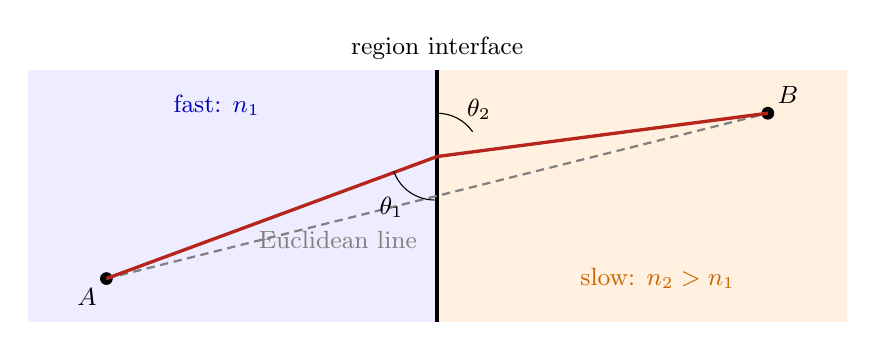
\begin{tikzpicture}[font=\small,x=1cm,y=1cm]
 \fill[blue!7] (0,0) rectangle (5.2,3.2);
 \fill[orange!12] (5.2,0) rectangle (10.4,3.2);
 \draw[very thick] (5.2,0)--(5.2,3.2) node[above] {region interface};
 \fill (1,.55) circle (2.3pt) node[below left] {$A$};
 \fill (9.4,2.65) circle (2.3pt) node[above right] {$B$};
 \draw[gray,densely dashed,thick] (1,.55)--(9.4,2.65) node[pos=.35,below] {Euclidean line};
 \draw[BrickRed,very thick] (1,.55)--(5.2,2.1)--(9.4,2.65);
 \draw[dotted] (5.2,1.2)--(5.2,2.9);
 \draw (4.65,1.91) arc[start angle=200,end angle=270,radius=.55];
 \draw (5.2,2.1) ++(0,.55) arc[start angle=90,end angle=35,radius=.55];
 \node at (4.62,1.45) {$\theta_1$};
 \node at (5.73,2.7) {$\theta_2$};
 \node[blue!70!black] at (2.4,2.75) {fast: $n_1$};
 \node[orange!80!black] at (8.0,.55) {slow: $n_2>n_1$};
\end{tikzpicture}
\caption{Piecewise-flat teaching model.  A path can be longer in amperes but
faster in time by spending more distance in the dynamically fast region.
Stationarity of the interface crossing gives the Snell condition.}
\label{fig:optical-pwa}
\end{figure}



This construction suggests an embedded approximation: precompute flat-region
segments, evaluate a small number of interface candidates, and verify every
segment against the original nonlinear flux map.  It is exact only for the
declared piecewise model.

\subsection{The earlier conformal square map under dynamics}

For \(w=z_\psi+\mathrm jz_q\) and \(\zeta=w^2\),
\[
 \dot\zeta=2w\dot w.
 \tag{28.6}
\]
The real part still exposes the difference of squares and the imaginary part
is proportional to torque.  Thus torque dynamics are visually direct.
However, the voltage-reachable body is multiplied by the state-dependent
Jacobian \(2w\); it collapses at \(w=0\), double-covers the plane away from the
origin, and generally introduces rather than removes metric variation.  The
map is useful for task visualization, not a generic geodesic flattening.

